\documentclass[12pt, a4paper]{article}

\usepackage[top=1in, bottom=1in, left=1in, right=1in]{geometry}
\usepackage[T1]{fontenc}
\usepackage[utf8]{inputenc}
\usepackage[protrusion=true,expansion=false]{microtype}
\usepackage{titlesec}
\usepackage{titling}
\usepackage{hyperref}
\usepackage{graphicx}
\usepackage{listings}
\usepackage{xcolor}
\usepackage{booktabs}
\usepackage{fancyhdr}
\usepackage{dirtree}
\usepackage{parskip}

\bibliographystyle{unsrt}

\setlength{\headheight}{13.6pt}
\addtolength{\topmargin}{-1.6pt}

% ── Hyperlink styling ────────────────────────────────────────────
\hypersetup{
    colorlinks=true,
    linkcolor=black,
    urlcolor=blue,
    citecolor=black
}

% ── Code listing style ───────────────────────────────────────────
\lstset{
    basicstyle=\ttfamily\small,
    backgroundcolor=\color{gray!10},
    frame=single,
    framerule=0.4pt,
    rulecolor=\color{gray!40},
    breaklines=true,
    numbers=left,
    numberstyle=\tiny\color{gray},
    keywordstyle=\color{blue!70},
    commentstyle=\color{green!50!black},
    stringstyle=\color{orange!80!black},
    showstringspaces=false,
    tabsize=4
}

% ── Section formatting ───────────────────────────────────────────
\titleformat{\section}
    {\large\bfseries}{\thesection.}{0.5em}{}[\titlerule]
\titleformat{\subsection}
    {\normalsize\bfseries}{\thesubsection}{0.5em}{}

% ── Header / Footer ──────────────────────────────────────────────
\pagestyle{fancy}
\fancyhf{}
\rhead{\small Mini Game Hub - Bash + Python}
\lhead{\small Dhruba Jyoti Panja(25B0945) Vishad Jain()}
\rfoot{\thepage}
\renewcommand{\headrulewidth}{0.4pt}

% ── Title block ──────────────────────────────────────────────────
\title{
    \vspace{-1cm}
    {\LARGE \textbf{MINI GAME HUB}} \\[0.4em]
    {\large SOFTWARE SYSTEMS LAB(SSL)} \\[0.1em]
    {\large CS 108}\\
    {\normalsize Project Report}
}
\author{
    Dhruba Jyoti Panja and Vishad Jain\\ \\[0.3em]
}
\date{\today}


\begin{document}

\maketitle
\thispagestyle{empty}
\vspace{1em}

% ── Abstract ────────────────────
\begin{abstract}
    This project is about a Mini board game we have made using python and bash. It is a completely offline 2 player game and till now, we have added 3 games in this hub namely - Tictactoe, Othello and Connect 4.
\end{abstract}

\newpage
\tableofcontents
\newpage

\section{External Libraries}

Here is a list of all libraries we are using to make this game. Hence, to run the game, these libraries should be installed in the system of these versions or higher. (Lower versions can also work though they are subjected to system failure)

\begin{table}[h!]
\centering
\begin{tabular}{lll}
\toprule
\textbf{Library / Tool} & \textbf{Version} & \textbf{Purpose} \\
\midrule
pygame       & 2.6.1 & Game window, rendering, event handling \\
numpy        & 1.26.4 & Board state representation, win or valid move detection \\
matplotlib   & 3.10.0 & Statistics charts and gauges in an aesthetic way \\

\bottomrule
\end{tabular}
\caption{External dependencies}
\end{table}


\section{Design \& Architecture}

Here is a high level description of the entire structure of the program and the reasons behind some key design decisions and their benefits in this overall journey of developing this project.

\subsection{Overall Structure}
    \subsubsection*{game.py}
The game.py is the engine of the entire program which handles the sequence of events through various parameters like
\begin{lstlisting}
    is_menu, fading, results, stats, etc
\end{lstlisting}

Apart from this, it has many classes like
\begin{lstlisting}
    TransitionManager, Button, Checkbox, Menu, Board
\end{lstlisting}
which facilitate coding complex things and reuses codes extensively. There are many functions in the Board class which is the main class that handles the sequencing of events of different screens by methods like
\begin{lstlisting}
    show_charts(), show_leaderboard(), show_results(), etc
\end{lstlisting}
These methods are calling functions like
\begin{lstlisting}
    draw_charts(), draw_gauges(), draw_leaderboard(), etc
\end{lstlisting}
which handle only the design part of the respective screens. This was an important decision to make which enables separation of function handling a particular screen into two - one for logistics and another for design. This enables easy future customizing of components and screens without interfering the basic program logics.

There are also 3 functions which are discussed in detail in the next section:
\begin{lstlisting}
    play(), win_check(), turn_change()
\end{lstlisting}
These functions are modified in respective game classes. The game.py handles the general common logistics for each and every game using these functions whose definitions are varied with each game.

\subsubsection*{games folder}
In the games folder, the respective game classes are written whose main job is to modify the three functions, play(), win\texttt{\_}check() and turn\texttt{\_}change() using other useful functions and variables.

\subsubsection*{pictures folder}
There is also a pictures folder which contains useful pictures which different .py files are pasting on the pygame screen.

\subsubsection*{\texttt{\_\_init\_\_}}
There are \texttt{\_\_init\_\_} in the home directory and in the games folder to enable importations of .py files within each other.

\subsubsection*{history.csv}
After the completion of any game, the results of the game is stored in history.csv in the format as follows:
\begin{lstlisting}
    DRAW/NOTDRAW,player 1,player 2,winner/NA,loser/NA,Date of play,Game name
\end{lstlisting}
Winner and Loser fields can be NA also in case of a draw.

\subsubsection*{main.sh}
VISHAD

\subsubsection*{leaderboard.sh and leaderboard.awk}
VISHAD



\subsection{Major Components}
\subsubsection{game.py}
\begin{itemize}
    \item{\textbf{Button class:} It manages all the necessities and parameters for a button. One simple example is as follows
    \begin{lstlisting}{language=python}
        b=Button(text,x,y,width,height,font: pygame.font, offset=0,style=None)
        b.draw(screen)
        if b.handle_event(event):
            #do some action if button clicked
            pass
    \end{lstlisting}
    Therefore, the draw manages all design properties of a button. The handle\texttt{\_}event enables hovering action and returns True if clicked. The assign function is to resize a button or alter any of its properties without deleting its memory or creating any new object.
    }
    \item{\textbf{Checkbox class:}
    It manages all the design and logistics for a checkbox along with a text and an additional radio button. In this class there is no option to remove the radio button because that functionality was never required in the project. Here, select function just marks the checkbox as selected and similarly deselect function marks it as unselected. The draw function manages its design and assign function just resets some useful parameters during resizing dynamically without making another object or removing the memory of whether it is selected or not.
    Usage:
    \begin{lstlisting}
        c=Checkbox(x, y, rect_width,text,idx,font_name="Consolas", radius=10)
        c.draw(screen,style=None)
        if box is selected:
            c.select()
        if box is unselected:
            c.deselect()
    \end{lstlisting}
    }
    \item{\textbf{Transition Manager: }
    This class handles the slowly darkening of screen when the user selects a game from menu and again slowly reappearing of the game screen. It is solely for this fading in and out animation. It is reused elsewhere also when any game ends.
    }
    \item{\textbf{Menu: } It is just for drawing the main menu and handling its buttons depending on which that particular game is executed}
    \item{\textbf{Board: } This is the main class which actually provides the functions for appearing of the background picture by page() function, appearing of any fashionable screen matching with the theme by fancy\texttt{\_}screen() function, drawing of results screen, leaderboard screen, displaying charts, display the final screen of playing again or quitting and finally, providing the function for implementing a special options button with customizable style for each and every game.\\
    In addition to the main functions, there are many helping functions which ease the coding part and shortens the code such as \texttt{draw\_hbar(), glow\_text(),\\ draw\_corner\_brackets() and draw\_gauge()}
    }
    \item{\texttt{\_\_main\_\_} :
    It handles the overall display of the pygame screen such as its title, icon and its initial witdth and height. It also manages the sequencing of screens to be displayed one after another in response to any event occurred. It redraws the screen every frame and handles when to close the pygame interface.
    }
   
\end{itemize}


\subsection{Key Design Decisions}
Some key design decisions are listed below to make the code reusable and easy to implement
\begin{itemize}
    \item{There was an initiative from our side from the very beginning that we should have sufficient modularity to reuse the codes but not so much that we are making unnecessary functions. So we have created game.py as the master file which govern the functions written in the code of other games. Hence, we started from the game.py and simultaneously relating the functions with one of the games, tictactoe.py while making it. We kept only functions and classes in tictactoe.py whose functioins are not even very much related to each other but makes a good correlation when combined with game.py}
    \item{We created a master class in game.py called 'Board' which handles all the design and logistics of common screens such as leaderboard, results, charts and the final screen but still made their design customizable with the game being played.}
    \item{There was an importation error while importing tictactoe.py,connect4.py and othello.py into game.py and importing game.py into their code because there was circulation importation happening. So we kept the main part of game.py into an if block.}
    \item{Separate classes of buttons, checkboxes and transitioning were made in game.py to easily modify their design and logistics with modularity. Also these were kept in game.py so that all of the games can access them in any quick making of components.}
    \item{For any particular screen, we have created atleast two functions like \texttt{draw\_charts()} and \texttt{show\_charts()} such that one handles the logistics and the other manages the design part. This is done so that we can change the design part whenever we wanted without hampering any change in the game logic.}
    \item{In Othello, since the game is of East\texttt{\-}Asian origin, we decided to have a theme on tigers and dragons with the title "Fangs vs Flames".}
    \item{Further, in Othello, due to the more convoluted nature of the game, we decided that it is important to have a log screen which shows incorrect attempts at placing tokens and informs when a player's turn is skipped}
    \item{For othello, we introduced a separate variable to test on 4×4 board so that the testing gets faster}
    \item{We have introduced multiple parameters based on which leaderboard is sorted. Hence we have introduced a priority to be set for all the options available and display them in leaderboard screen with numbers within checkboxes}
    \item{Introduced a style parameter changing the values of which, the colours and theme of many components like buttons, checkboxes, panels, borders can be set very conveniently.}
    \item{A separate options button is provided which enables each user to resign or just quit the game normally without resigning.}
\end{itemize}

\section{Features Implemented}

\subsection{Game Modes}
\begin{itemize}
    \item \textbf{Tic Tac Toe} — 10×10 board, 5 in a row win condition with cyberpunk theme.
    \item \textbf{Othello} — 8×8 board with the theme of "Fangs vs Flames".
    \item \textbf{Connect 4} — 7×7 board, 4 in a row win condition with steampunk theme.
\end{itemize}

\subsection{UI \& Visual Features}
\begin{itemize}
    \item ASCII art in Login page and Leaderboard
    \item Animated transition screen between menu and game
    \item Resizable window with fully responsive layout
    \item Introduced three different themes with an introduction to the theme by the transition screen
    \item Animations of flipping othello pieces, falling pieces of connect 4 and changing turns in tictactoe
    \item Dynamic re-numbering of the priority list in leaderboard screen while choosing the priority
    \item In tictactoe, all the individual cells are given hovering effect for better UI
    \item In Connect 4, a small pointer is added which traces the mouse location and its size increases a bit when a move is placed.
    \item In Othello, a separate log screen is provided which \begin{itemize}
        \item Maintains a record of all moves made
        \item Informs users of an invalid attempt at making a move
        \item Informs user if their turn has been skipped
    \end{itemize}
    \item An options button is provided which provides the user 4 options: \begin{itemize}
        \item Player 1 resigns
        \item Player 2 resigns
        \item Quit the game without any resigning
        \item Resume the game
    \end{itemize}
    \item After completion of any game, the background screen darkens and the winner or draw text appear with custom formatting and design
    \item Both options of displaying the matplotlib screen as a separate screen and pasting the graph on pygame screen are provided to the user and can be switched by setting \texttt{True} or \texttt{False} to the variable \texttt{self.showing}
    \item{Donut type of pie charts and gauges are given in matplotlib instead of standard graphs}
\end{itemize}

\subsection{Statistics \& Leaderboard}
\begin{itemize}
    \item Persistent game history stored in \texttt{history.csv}
    \item Sortable leaderboard with priority-column selection
    \item Reverse-sort toggle per column
    \item A default sorting order is also preserved
    \item Matplotlib statistics dashboard (gauge charts, bar chart, donut chart)
    \item Two different themes are provided for displaying Matplotlib charts: steampunk and cyberpunk
    \item Both options for displaying the charts on pygame screen and Matplotlib screen are provided
    \item Leaderboard is implemented via bash and ASCII art.
   
\end{itemize}

\subsection{Other Features}
\begin{itemize}
    \item {The styling of buttons are handmade to match the background suitably}
    \item The buttons and name-plates in connect 4 are made on images to match the background
    \item All the components and images are sized in proportions to the width and heights to make them resizable
    \item For long names of players, they are truncated as necessary to fit in name plates or boxes
\end{itemize}

\newpage
\section{Directory Structure}

\begin{figure}[h!]
\dirtree{%
.1 project-root/.
.2 \texttt{\_\_init\_\_}\DTcomment{Used for linking of py files}.
.2 game.py\DTcomment{Board base class, UI components, main loop}.
.2 report.tex\DTcomment{Contains the report of the entire project in .tex}.
.2 bibliography.bib\DTcomment{Contains the bibliography for certain things used in the project}.
.2 report.pdf\DTcomment{The pdf of the report of all features and our experience in the project}.
.2 leaderboard.sh\DTcomment{Shell script to generate sorted leaderboard}.
.2 leaderboard.awk\DTcomment{Awk script used by leaderboard.sh}.
.2 main.sh\DTcomment{Shell script to generate Login page}.
.2 README.md\DTcomment{A readme of how to access entire directory and the entry points of the user}.
.2 README.pdf\DTcomment{A readme of the initial directory structure}.
.2 requirements.txt\DTcomment{Lists all required external libraries to be installed}
.2 users.tsv\DTcomment{It stores all the registered users}.
.2 history.csv\DTcomment{Persistent match history log}.
.2 Makefile\DTcomment{Build / run targets}.
.2 games/\DTcomment{Contains the py files for all the games available}.
.3 \texttt{\_\_init\_\_}\DTcomment{Used for linking of py files}.
.3 tictactoe.py\DTcomment{Tic Tac Toe game logic and rendering}.
.3 othello.py\DTcomment{Othello game logic and rendering}.
.3 connect4.py\DTcomment{Connect 4 game logic and rendering}.
.2 pictures/\DTcomment{Contains all pictures to be included in the game or useful}.
.3 background4.png\DTcomment{Background image of main menu}.
.3 black.png\DTcomment{One type of piece in connect 4}.
.3 blue.png\DTcomment{Another type of piece in connect 4}.
.3 connect4.png\DTcomment{Background image of connect 4}.
.3 icon.png\DTcomment{Icon displayed at top of pygame window}.
.3 icon1.png\DTcomment{An icon of player 1 for connect 4}.
.3 icon2.png\DTcomment{An icon of player 2 for connect 4}.
.3 plate.png\DTcomment{Plate on which player names are pasted}.
.3 player1.png\DTcomment{Plate with full formatted text of Player 1}.
.3 player2.png\DTcomment{Plate with full formatted text of Player 2}.
.3 tictactoe.png\DTcomment{Background image for tictactoe}.
.3 plot.png\DTcomment{Image saving the plot drawn by Matplotlib}.
.3 black\texttt{\_}token.jpeg\DTcomment{One token for Othello}.
.3 white\texttt{\_}token.jpg\DTcomment{Another token for Othello}.
.3 othello.jpg\DTcomment{Background image for Othello}.
}
\end{figure}


\section{Installation \& Setup}

\subsection{Requirements}
Python 3.10+ is required. Install all dependencies with:

\begin{lstlisting}[language=bash]
pip install -r requirements.txt
\end{lstlisting}

\noindent\texttt{requirements.txt} contains:

\begin{lstlisting}
pygame>=2.0
numpy>=1.21
matplotlib>=3.5
\end{lstlisting}

\section{Usage}

\subsection{Running the Project}

\begin{lstlisting}[language=bash]
python game.py <player1_name> <player2_name>
# example:
python game.py Alice Bob
\end{lstlisting}

OR if you have python3 in your system then you can also run:
\begin{lstlisting}[language=bash]
python3 game.py <player1_name> <player2_name>
# example:
python game.py Alice Bob
\end{lstlisting}

\subsection{Controls \& Interaction}
\begin{itemize}
    \item \textbf{Menu} — Click a game button to select and launch a game or click the close button to quit. You can also use the maximize button to maximize the screen.
    \item \textbf{In-game} — Click a cell / column to make a move. Some graphics animation will be related to your action for better experience.
    \item \textbf{Options} — Click the OPTIONS button (bottom-left) to resign,
          quit, or resume.
    \item \textbf{Results screen} — Press \texttt{SPACE} to continue to
          the leaderboard.
    \item \textbf{Leaderboard} — Select and prioritise sort columns,
          toggle reverse, then click Generate to generate the leaderboard in bash or click Visualize to see charts and graphs for a better visualization of the statistics.
    \item \textbf{Charts} - Click QUIT to exit the game and close the pygame interface or click MAIN MENU to return to the menu and play again
\end{itemize}
\newpage
\subsection{Screenshots}
% Include screenshots here — replace filenames with your actual files
\begin{figure}[h!]
    \centering
    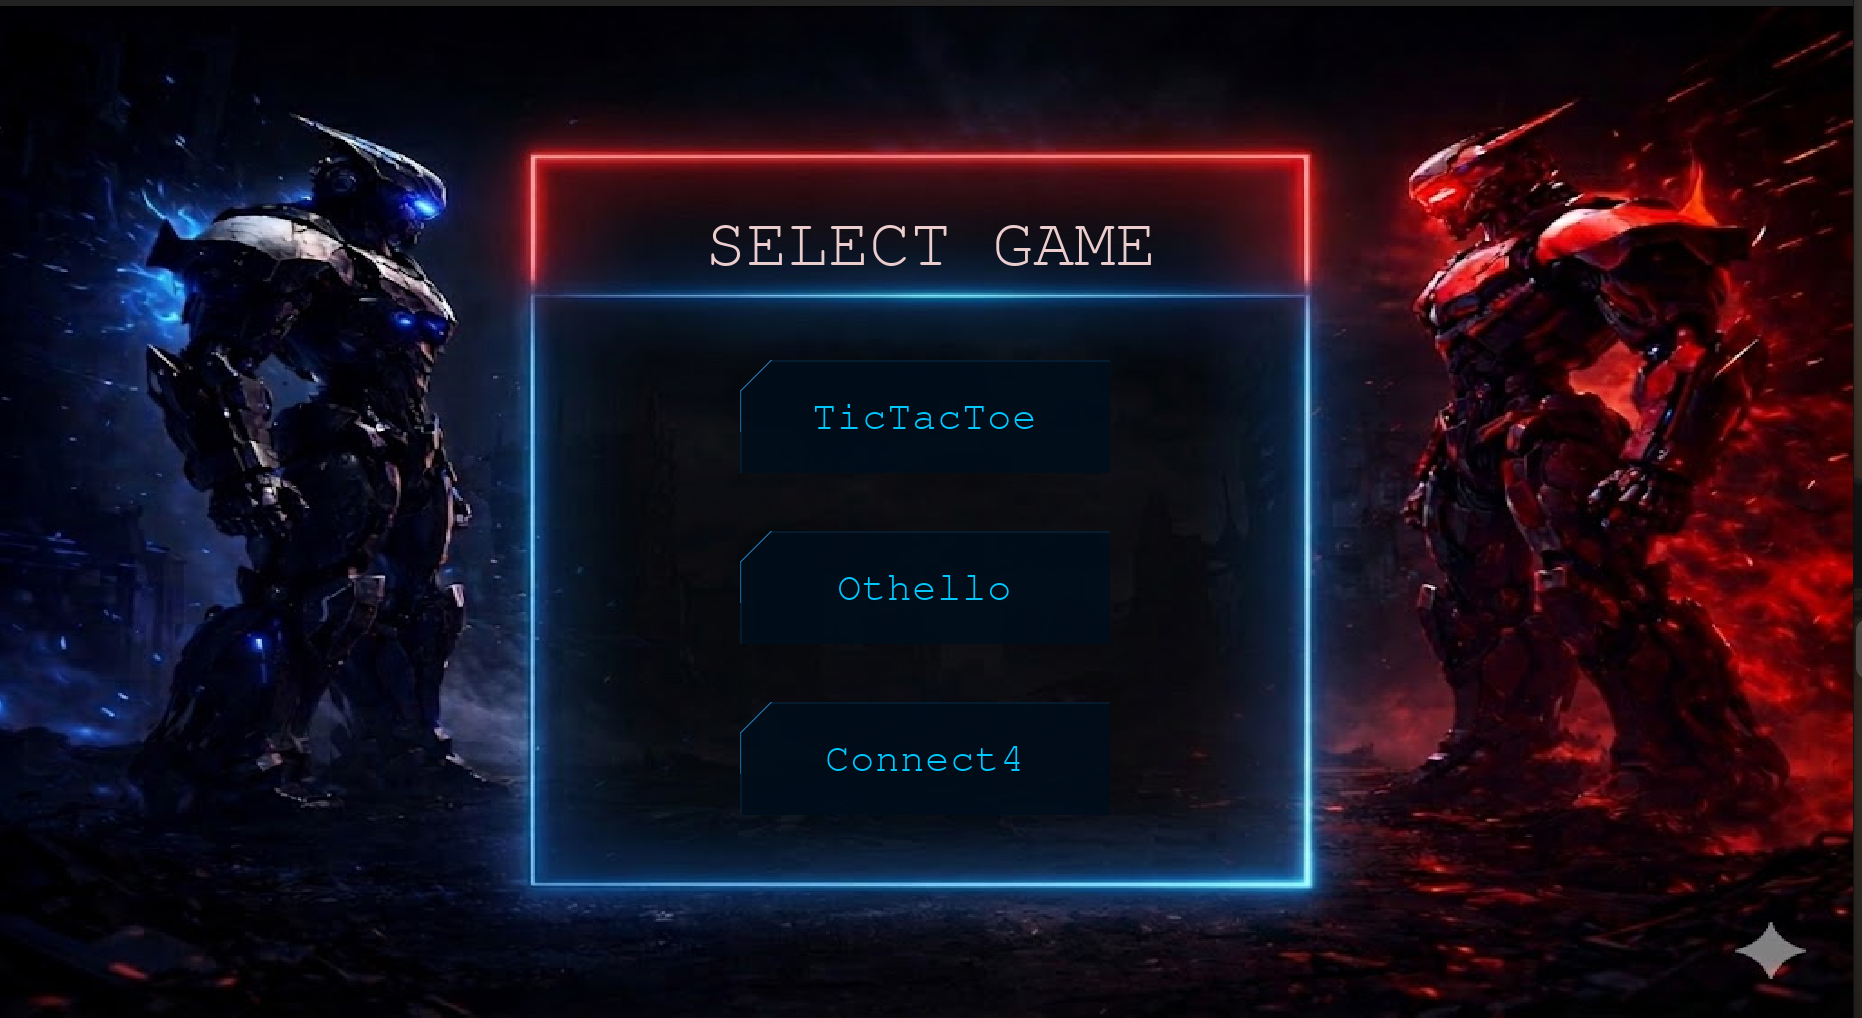
\includegraphics[width=0.8\textwidth]{pictures/MainMenu.png}
    \caption{Main menu screen}
\end{figure}

\begin{figure}[h!]
    \centering
    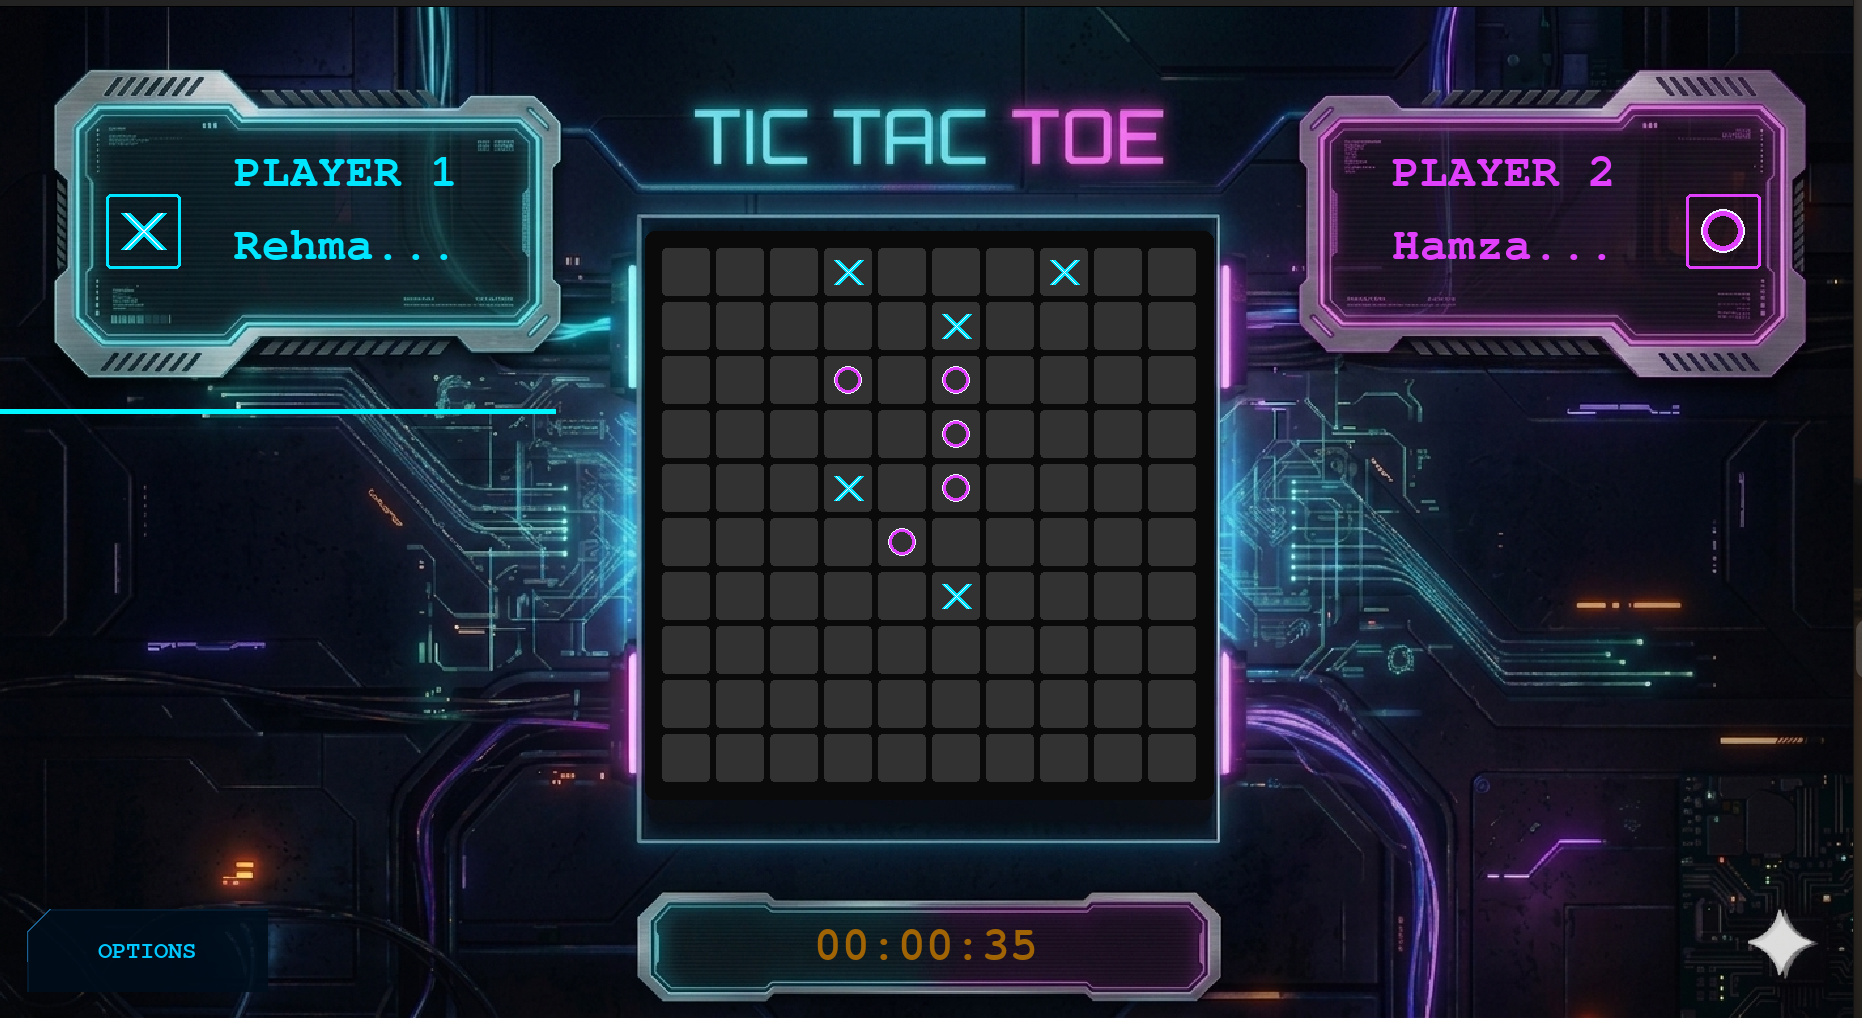
\includegraphics[width=0.8\textwidth]{pictures/TicTacToe_gameplay.png}
    \caption{In-game screen (TicTacToe)}
\end{figure}

\begin{figure}[h!]
    \centering
    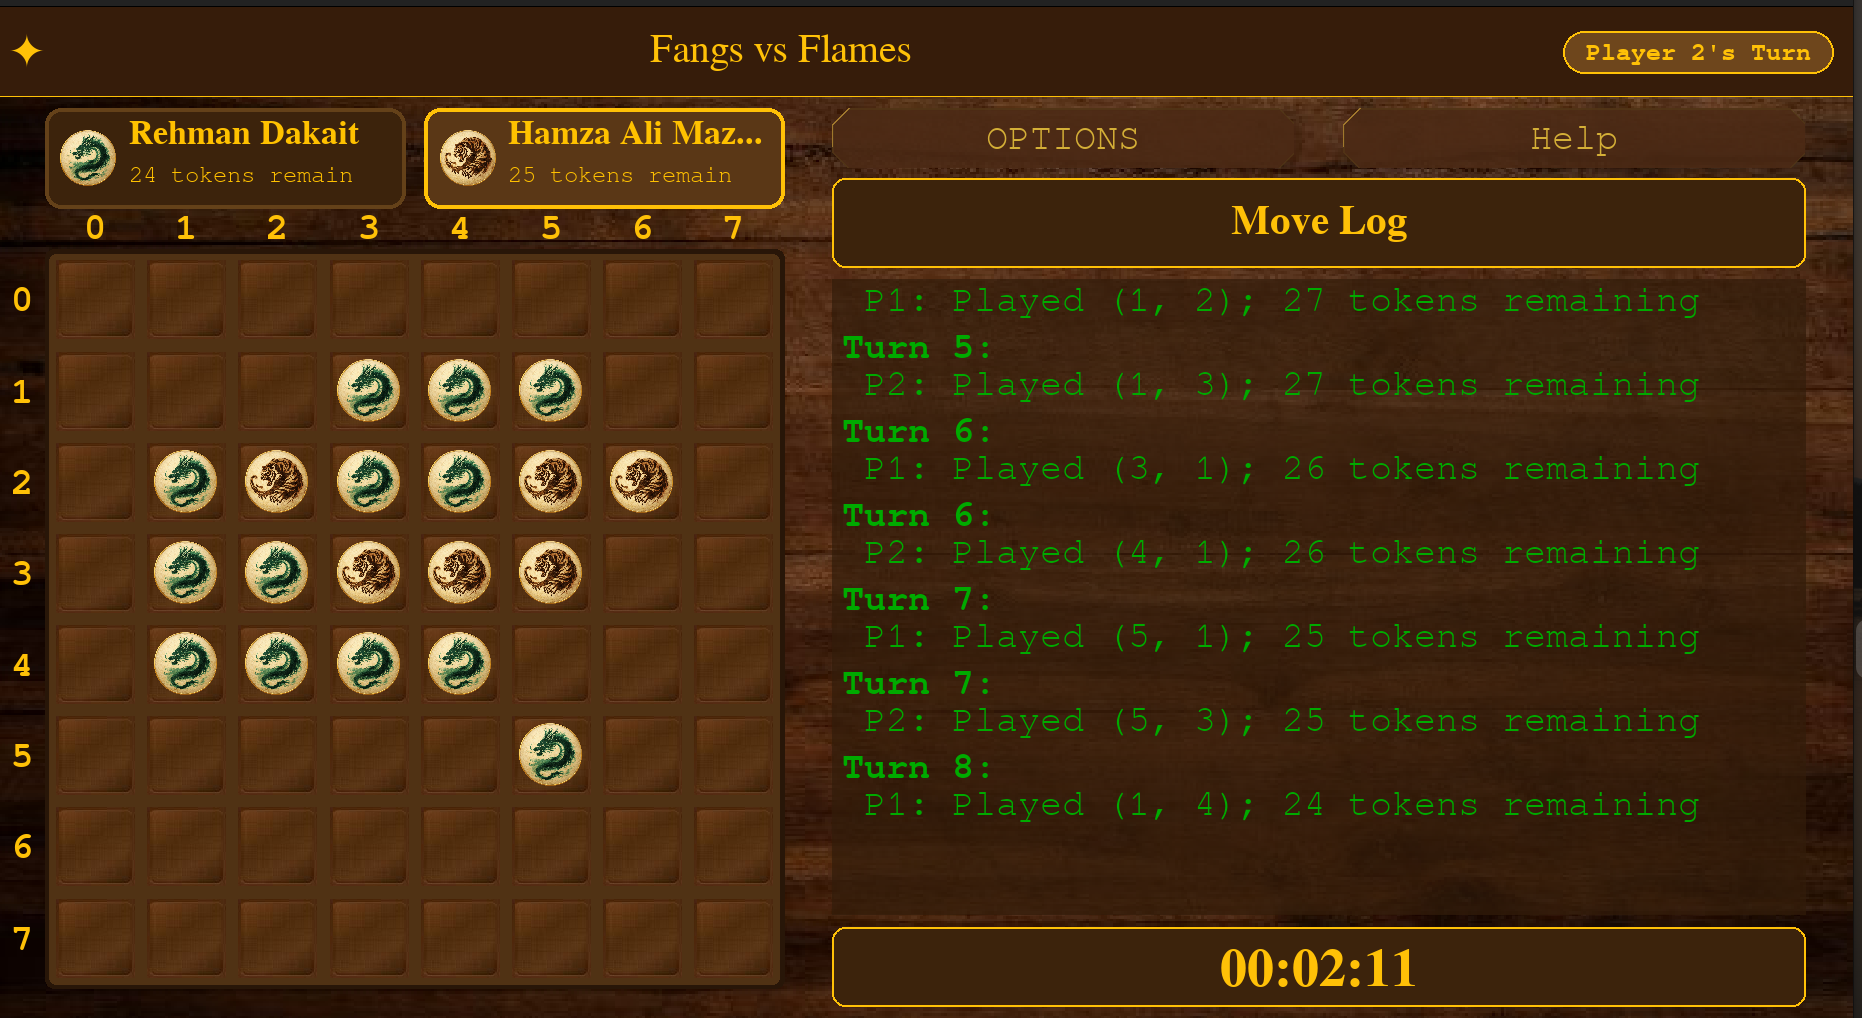
\includegraphics[width=0.8\textwidth]{pictures/Othello_gameplay.png}
    \caption{In-game screen (Othello)}
\end{figure}

\begin{figure}[h!]
    \centering
    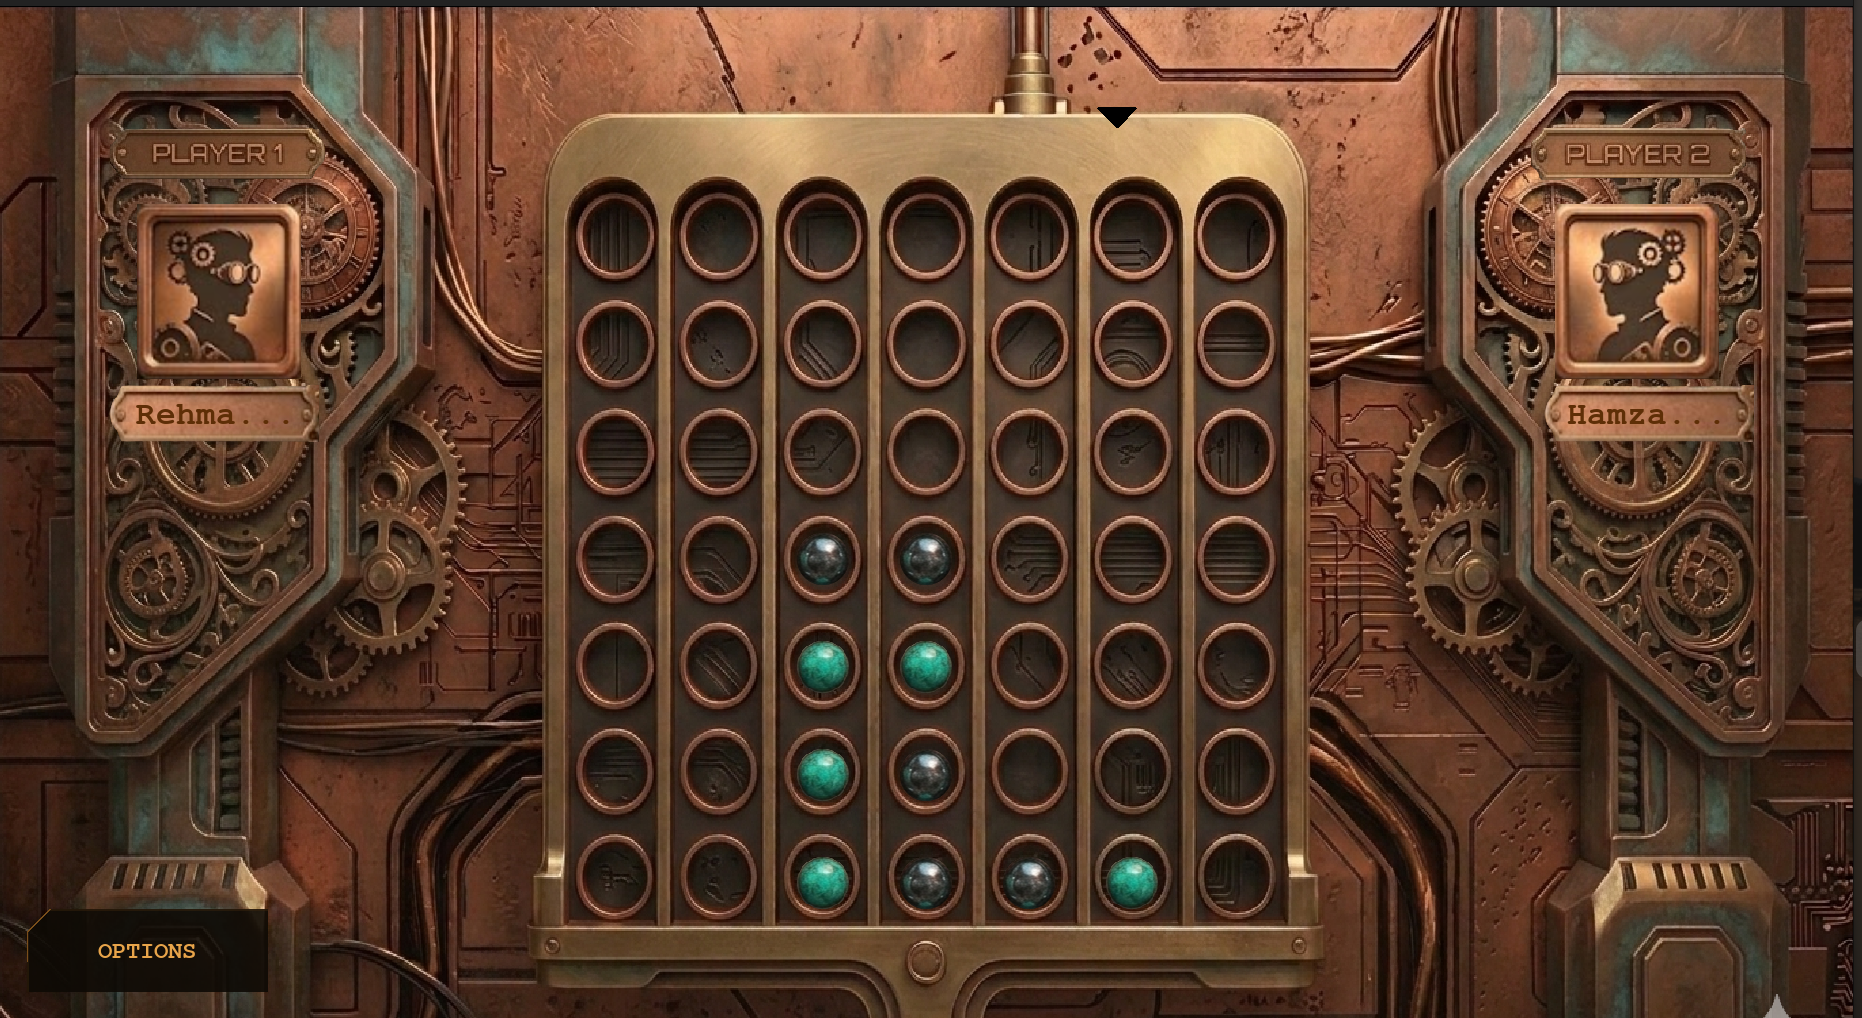
\includegraphics[width=0.8\textwidth]{pictures/Connect4_gameplay.png}
    \caption{In-game screen (Connect 4)}
\end{figure}
\newpage
\section{Retrospective}

\subsection{Challenges Faced}
\begin{itemize}
    \item \textbf{Responsive resizing} — Making every UI element
          scale correctly on \texttt{VIDEORESIZE} required auditing
          every hardcoded pixel value and switching to fractional
          coordinates relative to \texttt{screen.get\_size()}.
    \item \textbf{Custom Designing} — It was tiring to design each and every thing differently with a different theme and at the same time try to reuse the code as much as possible
    \item \textbf{Animation} — It way quite a hardwork to make indicator variables and a starting time stamp storing variable for each and every animation and code it correctly with the correct function of time to make the animation smooth and elegant
    \item \textbf{Formatting of text} — Making several panels with different alphas for blitting a simple text to make it glow on the screen
    \item Maintaining appropriate scrolling upon resizing
    \item Finding the correct color for different things and their correct positioning and sizes
\end{itemize}

\subsection{What Went Well}
\begin{itemize}
    \item A seemingly good game finally with a decent enough GUI according to us
    \item A lot of hardwork of past two months. Slowly building small pieces and when finally bringing everything together, it makes quite a complete picture
    \item We got to learn many concepts of pygame, bash, encryption, etc.
\end{itemize}

\subsection{What I Would Do Differently}
\begin{itemize}
    \item If more time was there then we would have added more games like chess (we wanted to add it)
    \item Probably, some more interesting animations could have been given
\end{itemize}


\nocite{*}
\bibliography{bibliography}

\end{document}
